% vim: set ts=2 sw=2 noet spell:

\chapter{Implementation}

\section{Overview}

% TODO: quelle https://wiki.gnuradio.org/
For the simulation task and after for the Hardware part, the open-source Software GNU Radio has been chosen. This software uses toolboxes for signal processing systems too simulate or/and implement a software-defined radio, based on Python and some C++ implementations for some rapid-application-development environments. The toolboxes can simply, with the help of the graphical user interface, used by drag-and-drop. The Boxes are used to write applications, to receive or to transmit date for a digital system. Some blocks like different filters, channel codes or demodulator elements and a lot more are already implemented. For missing application new elements can be added by coding own blocks. With the help of the GNU Radio software those toolboxes can easily get connected to each other, creating data streams. 

\section{Sender chain}
\subsection{Data source}

%% TODO: replace with file file
In this simulation a random source has been chosen.

\subsection{Modulation}

The constellation modulator block is used for a root-raised-cosine-filtered basis modulation. The block gives an input of a byte stream as complex modulated signal in the baseband back. 
Further more it's possible to chose the modulation type here, in this example it is 16QAM, but QPSK, 8PSK and BPSK would also be possible.

\section{Receiver chain}

\subsection{Envelope detector}

\paragraph{Polyphase Clock Sync}
%% To Do : nochmals anschauen ob dieese erklärung verständlich ist und richtig interpretiert wurde.
With the the polyphase clock sync the symbols can be synchronized by preforming a time synchronization with the help of multiple filterbanks. For that the derivation of the filtered signal should be minimized whish turns to a better SNR. This works with the help of two filterbanks, one of them contains the filters of the signal adapted to the pulse shaping with several phases. The other contains its derivative. So in the time domain it has a sinc shape, for the output Signal the sinc peak should be on a sample, with the fact that sinc(0) = 1 and sinc(0)' = 0 an error signal can be generated which tells how far away from the peak it is. This error Signal should be zero this is possible with the help of a loop second order whish constants the number of the filterbank and the rate. This rate is generated because of the clock difference between the transmitter and reviver to synchronies the receiver the filter goes through the phases. For the output one sample per symbol is enough.

\paragraph{Equalizer}

\paragraph{Costas Loop}

The Costas Loop is used for frequency and phase adjustment it locks the center frequency of the signal additional it converts it back to de baseband.  For different modulation types different orders of the loop had to be chosen 

\paragraph{Constellation decoder}

From the complex space the constellation points are decode to bits.

\subsection{Frame synchronization}

\begin{figure}
	\centering
	% vim:ts=2 sw=2:
\begin{tikzpicture}[
		brace/.style = {
			decorate,
			decoration = {
				calligraphic brace,
				amplitude = 3mm,
				raise = 1mm,
				mirror,
			},
			very thick,
			pen colour = {black} 
		},
	]
	\matrix[
		column sep = -1pt,
		nodes = {
			draw, rectangle, very thick,
			minimum height = 12mm,
			text width = 20mm,
			align = center,
		},
	]{
		\node[] {Preamble \\ \(k\) Bytes}; &
		\node[fill=lightgray!20] (pad) {Padding \\ 1 Bit}; &
		\node[fill=red!10] (id) {ID \\ 5 Bits}; &
		\node[fill=red!10] {Length \\ 21 Bits}; &
		\node[fill=red!10] (par) {Parity \\ 5 Bits}; &
		\node[] {Payload \\ \(\ell\) Bytes}; \\
		% \node{Padding }; \\
	};

	\draw[brace] (id.south west) --
		node[midway, below = 5mm] {(31, 26) Hamming ECC}
		(par.south east);

	% \draw[brace] (par.north east) --
	% 	node[midway, above = 5mm] {4 Bytes}
	% 	(pad.north west);

\end{tikzpicture}

	\caption{
		Structure of framed data packets used in the implementation.
		\label{fig:dataframe}
	}
\end{figure}

To compute the empirical \emph{bit error rate} (BER) of the setup, the data has to be framed on by the sender and the bitstream synchronized on the receiver side. The structure of a data packed used in the implementation is shown in \figref{fig:dataframe}. A frame begins with an user specified \(k\)-byte preamble, that in the current implementation serves as synchronization pattern. Another use case for the preamble sequence could be to introduce channel estimation pilot symbols. Following the preamble are 4 bytes encoded using a (31, 26) Hamming code (plus 1 padding bit), that contain metadata about the packet, namely payload ID and payload length. Because the payload length in bytes is encoded in 21 bits, the maximum payload size is 2 MiB, which together with 32 possible unique IDs gives a maximum data transfer with unique frame headers of 64 MiB. These constraints are a result of decisions made to keep the implementation simple.

On the receiver side the bitstream is synchronized using a XOR correlator. To find the synchronization delay \(d\) (in samples) the XOR correlator computes the binary cross correlation
\begin{equation} \label{eqn:binary-xcorr}
	R_{\vec{m}\vec{p}} = N - \sum_i (\vec{m} \oplus \vec{p})_i
\end{equation}
between the synchronization bit pattern \(\vec{p}\) and a shift register \(\vec{m}(n)\) of the same length \(N\). Put into words \eqref{eqn:binary-xcorr} subtracts the number bits that differ between \(\vec{m}\) and \(\vec{p}\) from the length of the registers. Thus if all bits are equal, the difference is zero and the correlations has a maximum value of \(N\). The task of the correlator is then to find the delay / skip such that the pattern maches, i.e.
\begin{equation}
	d = \argmax_n \big( R_{\vec{m}\vec{p}}(n) \big)
		= \argmax_n \left( N - \sum_i (\vec{m}(n) \oplus \vec{p})_i \right)
	.
\end{equation}

Once the bit stream is synchronized, the packets are deframed and the payloads compared to a local copy of the sent data to compute the BER, again by XOR'ing the data blocks and counting the bit that are set. Further details are discussed in \S\ref{sec:ber}.

\section{Channel simulations}

Here its possible to add some AWGN noise in the channel line. Different parameters can be changed like the noise voltage, time or the frequency offset.

\skelpar[5]{
	Discuss the multitap FIR model we used. How it is possible to set the delay etc. Also mathematics for the interpolation.
}

%To get a basic line for further simulations a 16QAM has been made. The results of this simulation are shown in \figref{fig:simul16QAM} and \figref{fig:simul16QAM_1} as the red Signal. In \tabref{tab:modulation_settings} some importer Parameter settings for a different modulation scheme are mentioned.
%
%A FIR-Filter was added in the Channel to create a time delay between tow paths. In \figref{fig:simul16QAM} the result includes a direct path and a delayed one. In the plot of \figref{fig:simul16QAM_1} the transmission line dosn't include a direct path. %It's impotent to mention that the delay should be smaller than the symbol rate or a multiple of it. (Stimmt dies , not sure any more)
%
%For the a first simulation with some fading the 16QAM simulation model has been extended with a FIR-Filter in the Chanel. The results of this simulation are shown in \figref{fig:simul16QAM} and \figref{fig:simul16QAM_1} as the blue Signal.

\subsection{Fading}
%TO DO: übersetzen 
Für das veranschaulichen des Fading effekts wurde ein eigener Block kreaiert und in den Channel implementiert. Dieser Block basiert auf einem FIR Filter. Es kann mit direcktem Pfad oder ohne dargestellt werden ( Line of Side ). Mit Hilfe dieses Filters wird die Verspätung der nebenpfaden dargestellt. Es ist möglich beliebig viele dieser Pfade mit unterschiedlicher stärke zu simulieren.

% Bild einfügen 
\subsubsection{Fractional Delay}
Problem Werte nur auf dem Sample übermitelt und keine dazwischen.




\section{Hardware}

As Hardware we chosen the USRP B210 from Ettus Research, with the following specifications shown in \tabref{tab:USRP B210 specifications}. Because this SDR is more than enough for our requires.

For the Hardware setup up some changes are made in the file from the 16QAM simulation to fit with the SDRs. For the first test a coaxial cable was used as transmission line, after the cabel were been replaced with two antennas. The gnu radio block scheme is shown in \figref{fig:simul16QAM_Hardware_Aufbau}. The results for s anntena set uo with a transmission line of 20cm  are plotted in \figref{fig:simul16QAM__Hardware}.

Instead of the channel modeling block the USRP blocks are used. The sink as transmitter and the source as resiver.  The Signal is sended on a center frequency of 2.4GHz.

\subsection{Empirical BER} \label{sec:ber}

\subsection{Measurements}

%
%
%

\begin{figure}
	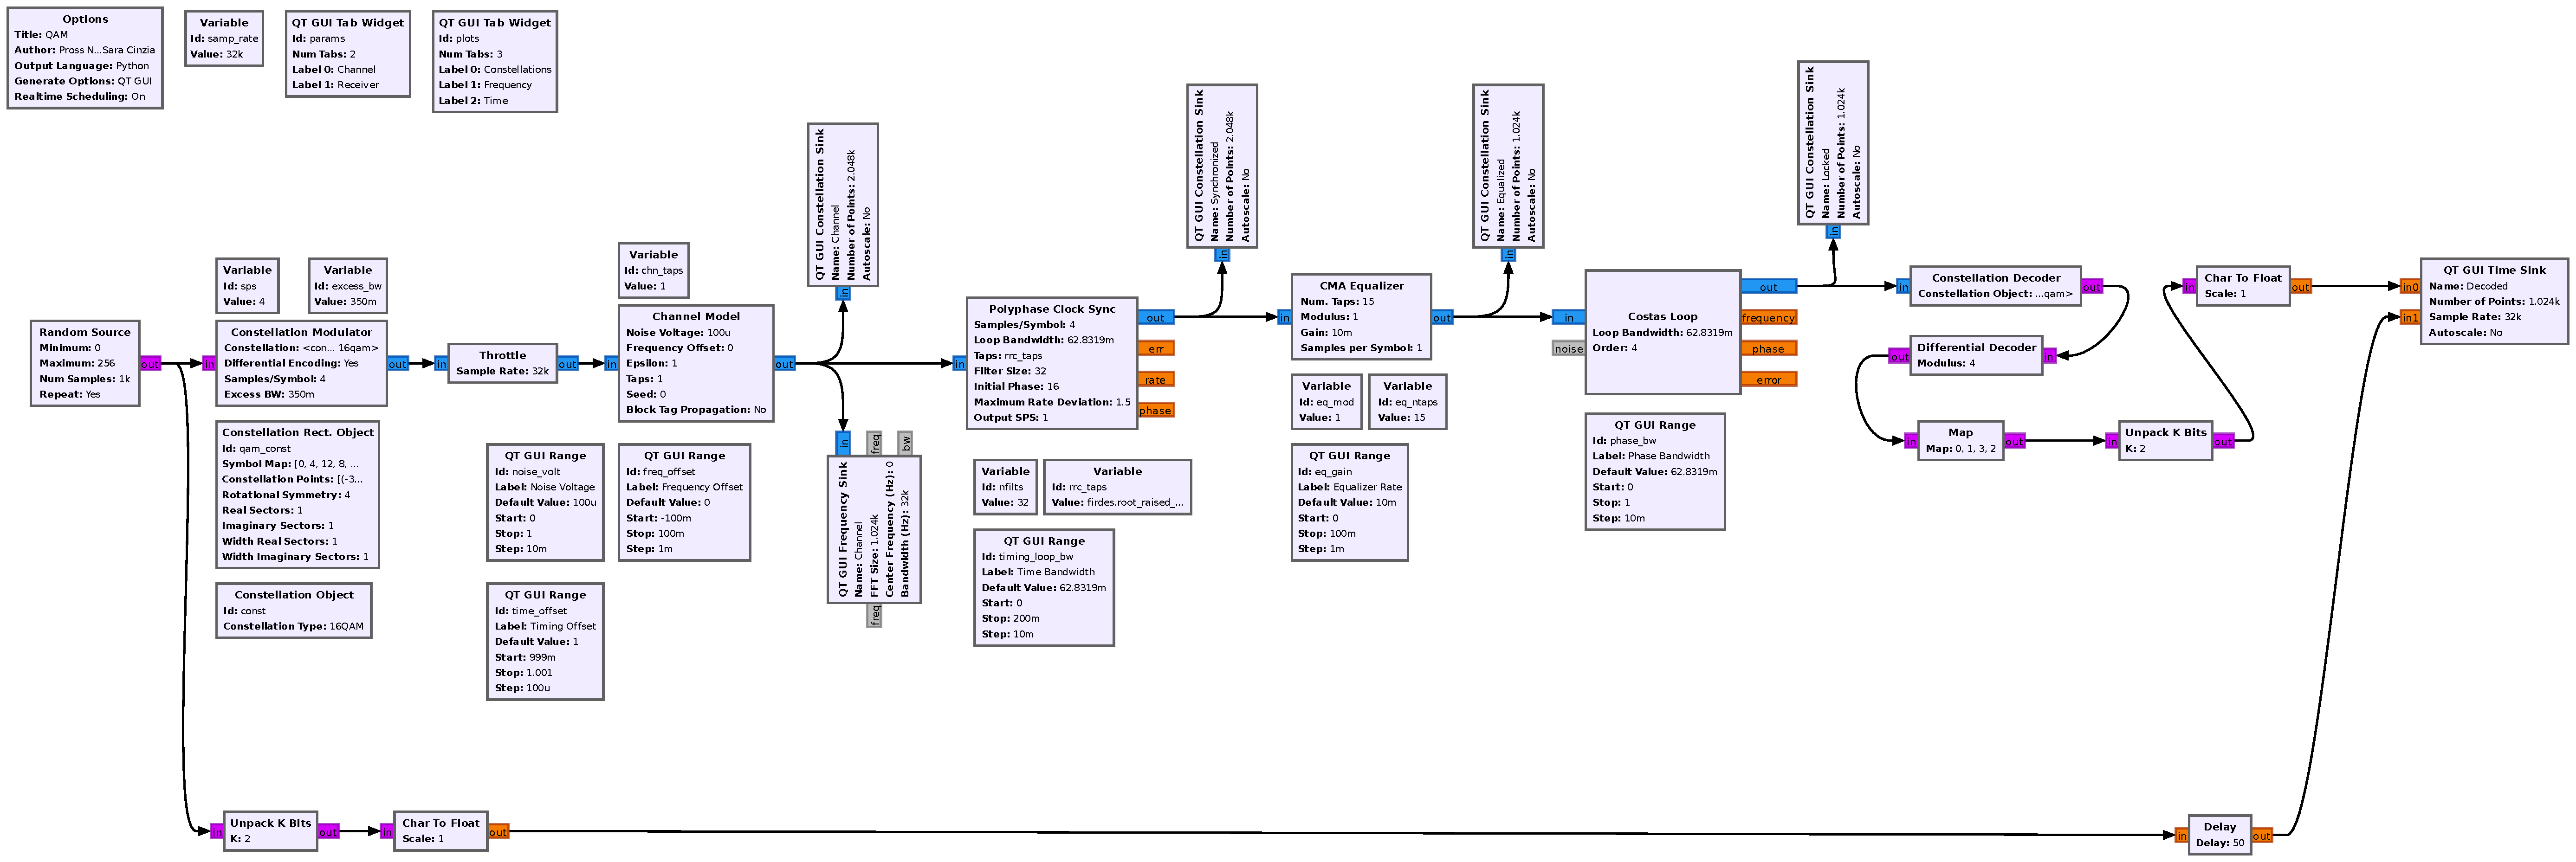
\includegraphics[width=\linewidth]{./figures/pdfs/qam_nogui.pdf}
	\caption{GNU Radio Blocks}
	\label{fig:simul16QAM_block}	
\end{figure}

\begin{figure}
	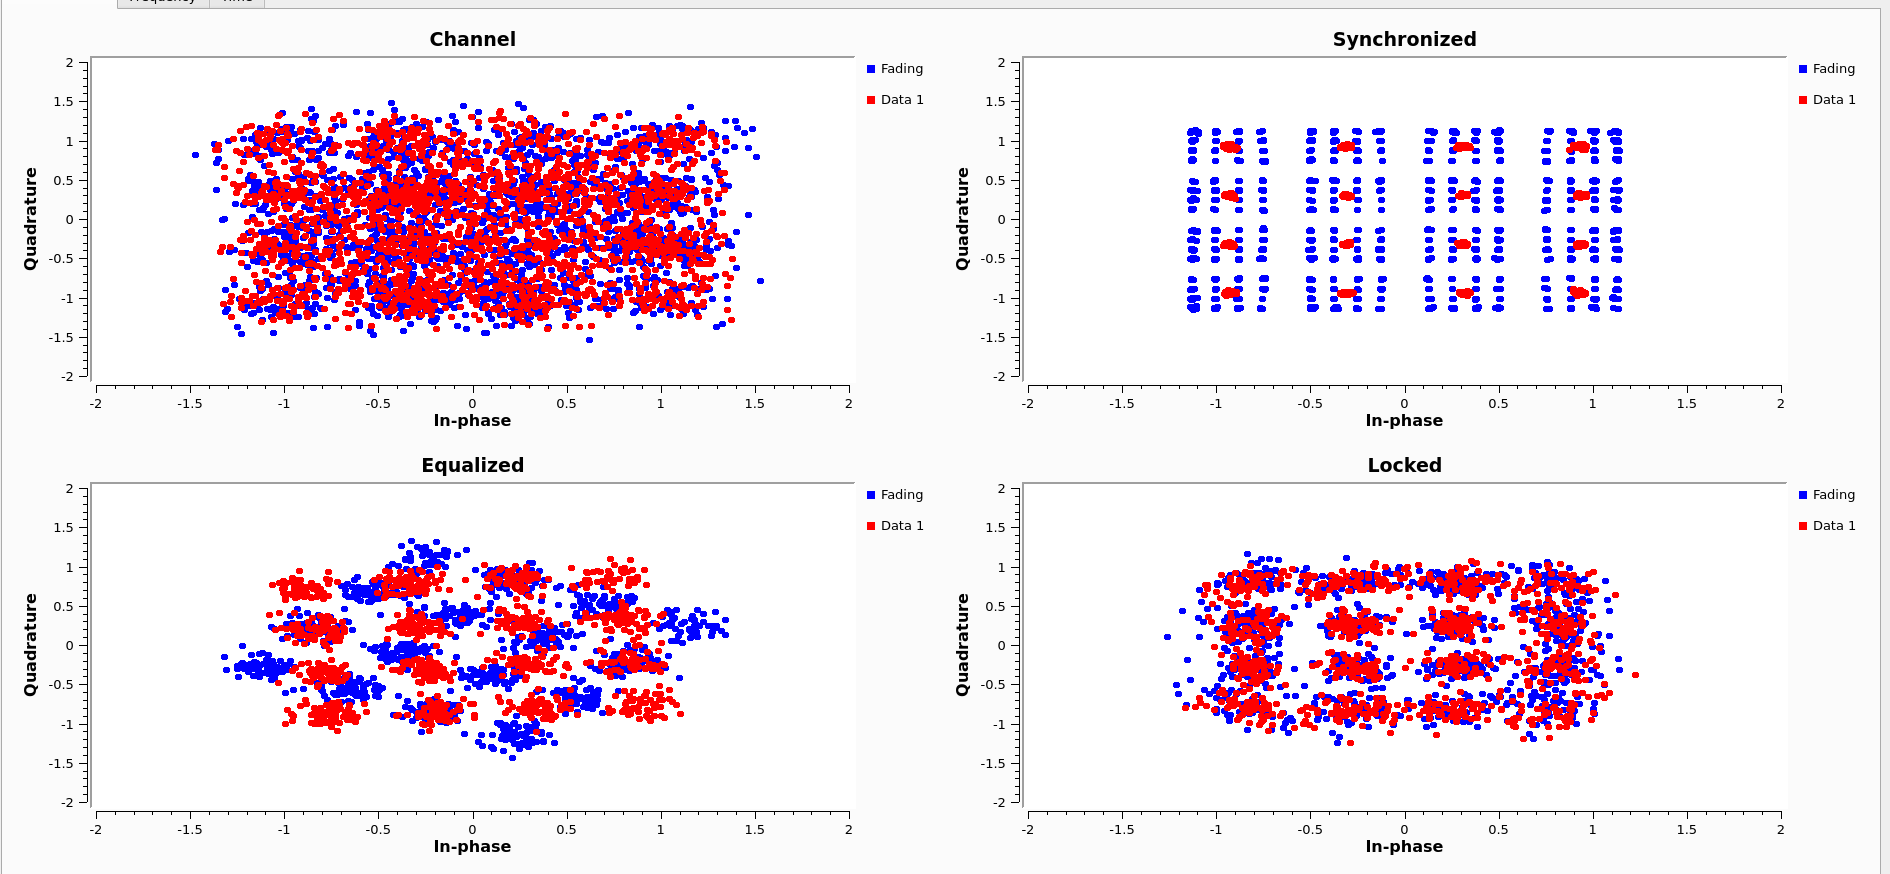
\includegraphics[width=\linewidth]{./figures/screenshots/QAM16_Fading_2.png}
	\caption{Simulation results}
	\label{fig:simul16QAM}	
\end{figure}

\begin{figure}
	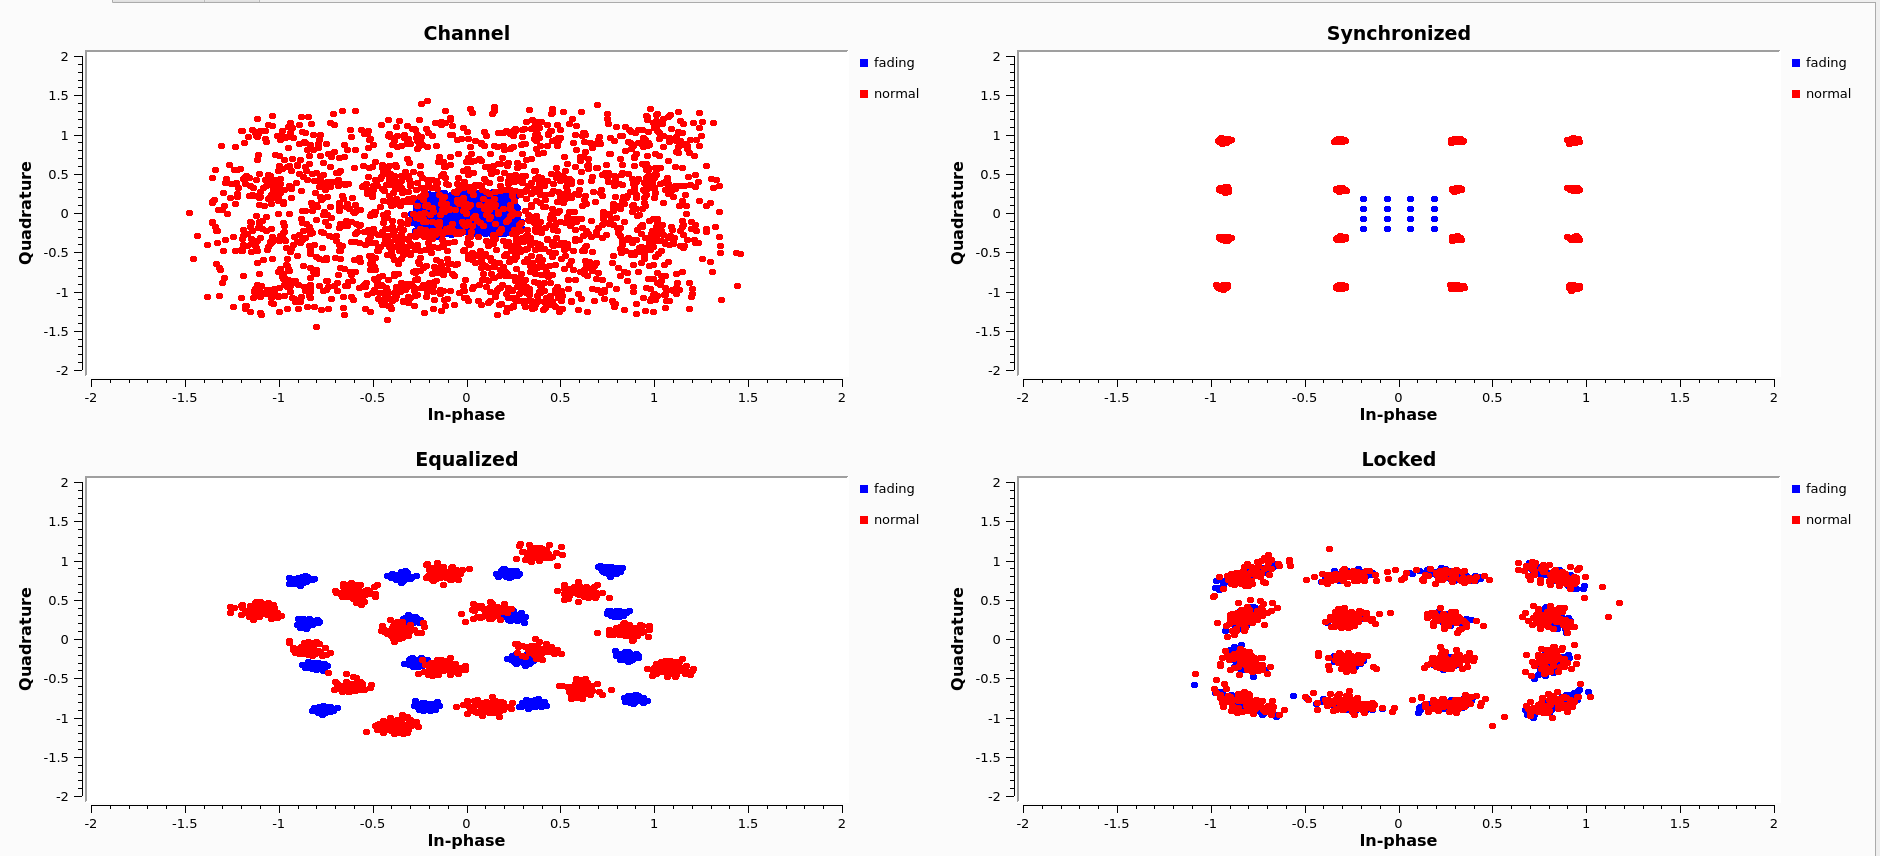
\includegraphics[width=\linewidth]{./figures/screenshots/QAM16_Fading_2_.png}
	\caption{Simulation results}
	\label{fig:simul16QAM_1}	
\end{figure}

\begin{table}[]
	\centering
	\caption{Modulation settings for different scheme}
	\begin{tabular}{ccc}
		\toprule
		Modulation Scheme & Samples per Symbol & Costas Loop Order\\
		\midrule
		BPSK  & 1 & 2 \\
		QPSK  & 2 & 4 \\
		8PSK  & 3 & 8 \\
		16QAM & 4 & 4 \\
		\bottomrule
	\end{tabular}
	\label{tab:modulation_settings}
\end{table}

\begin{figure}
	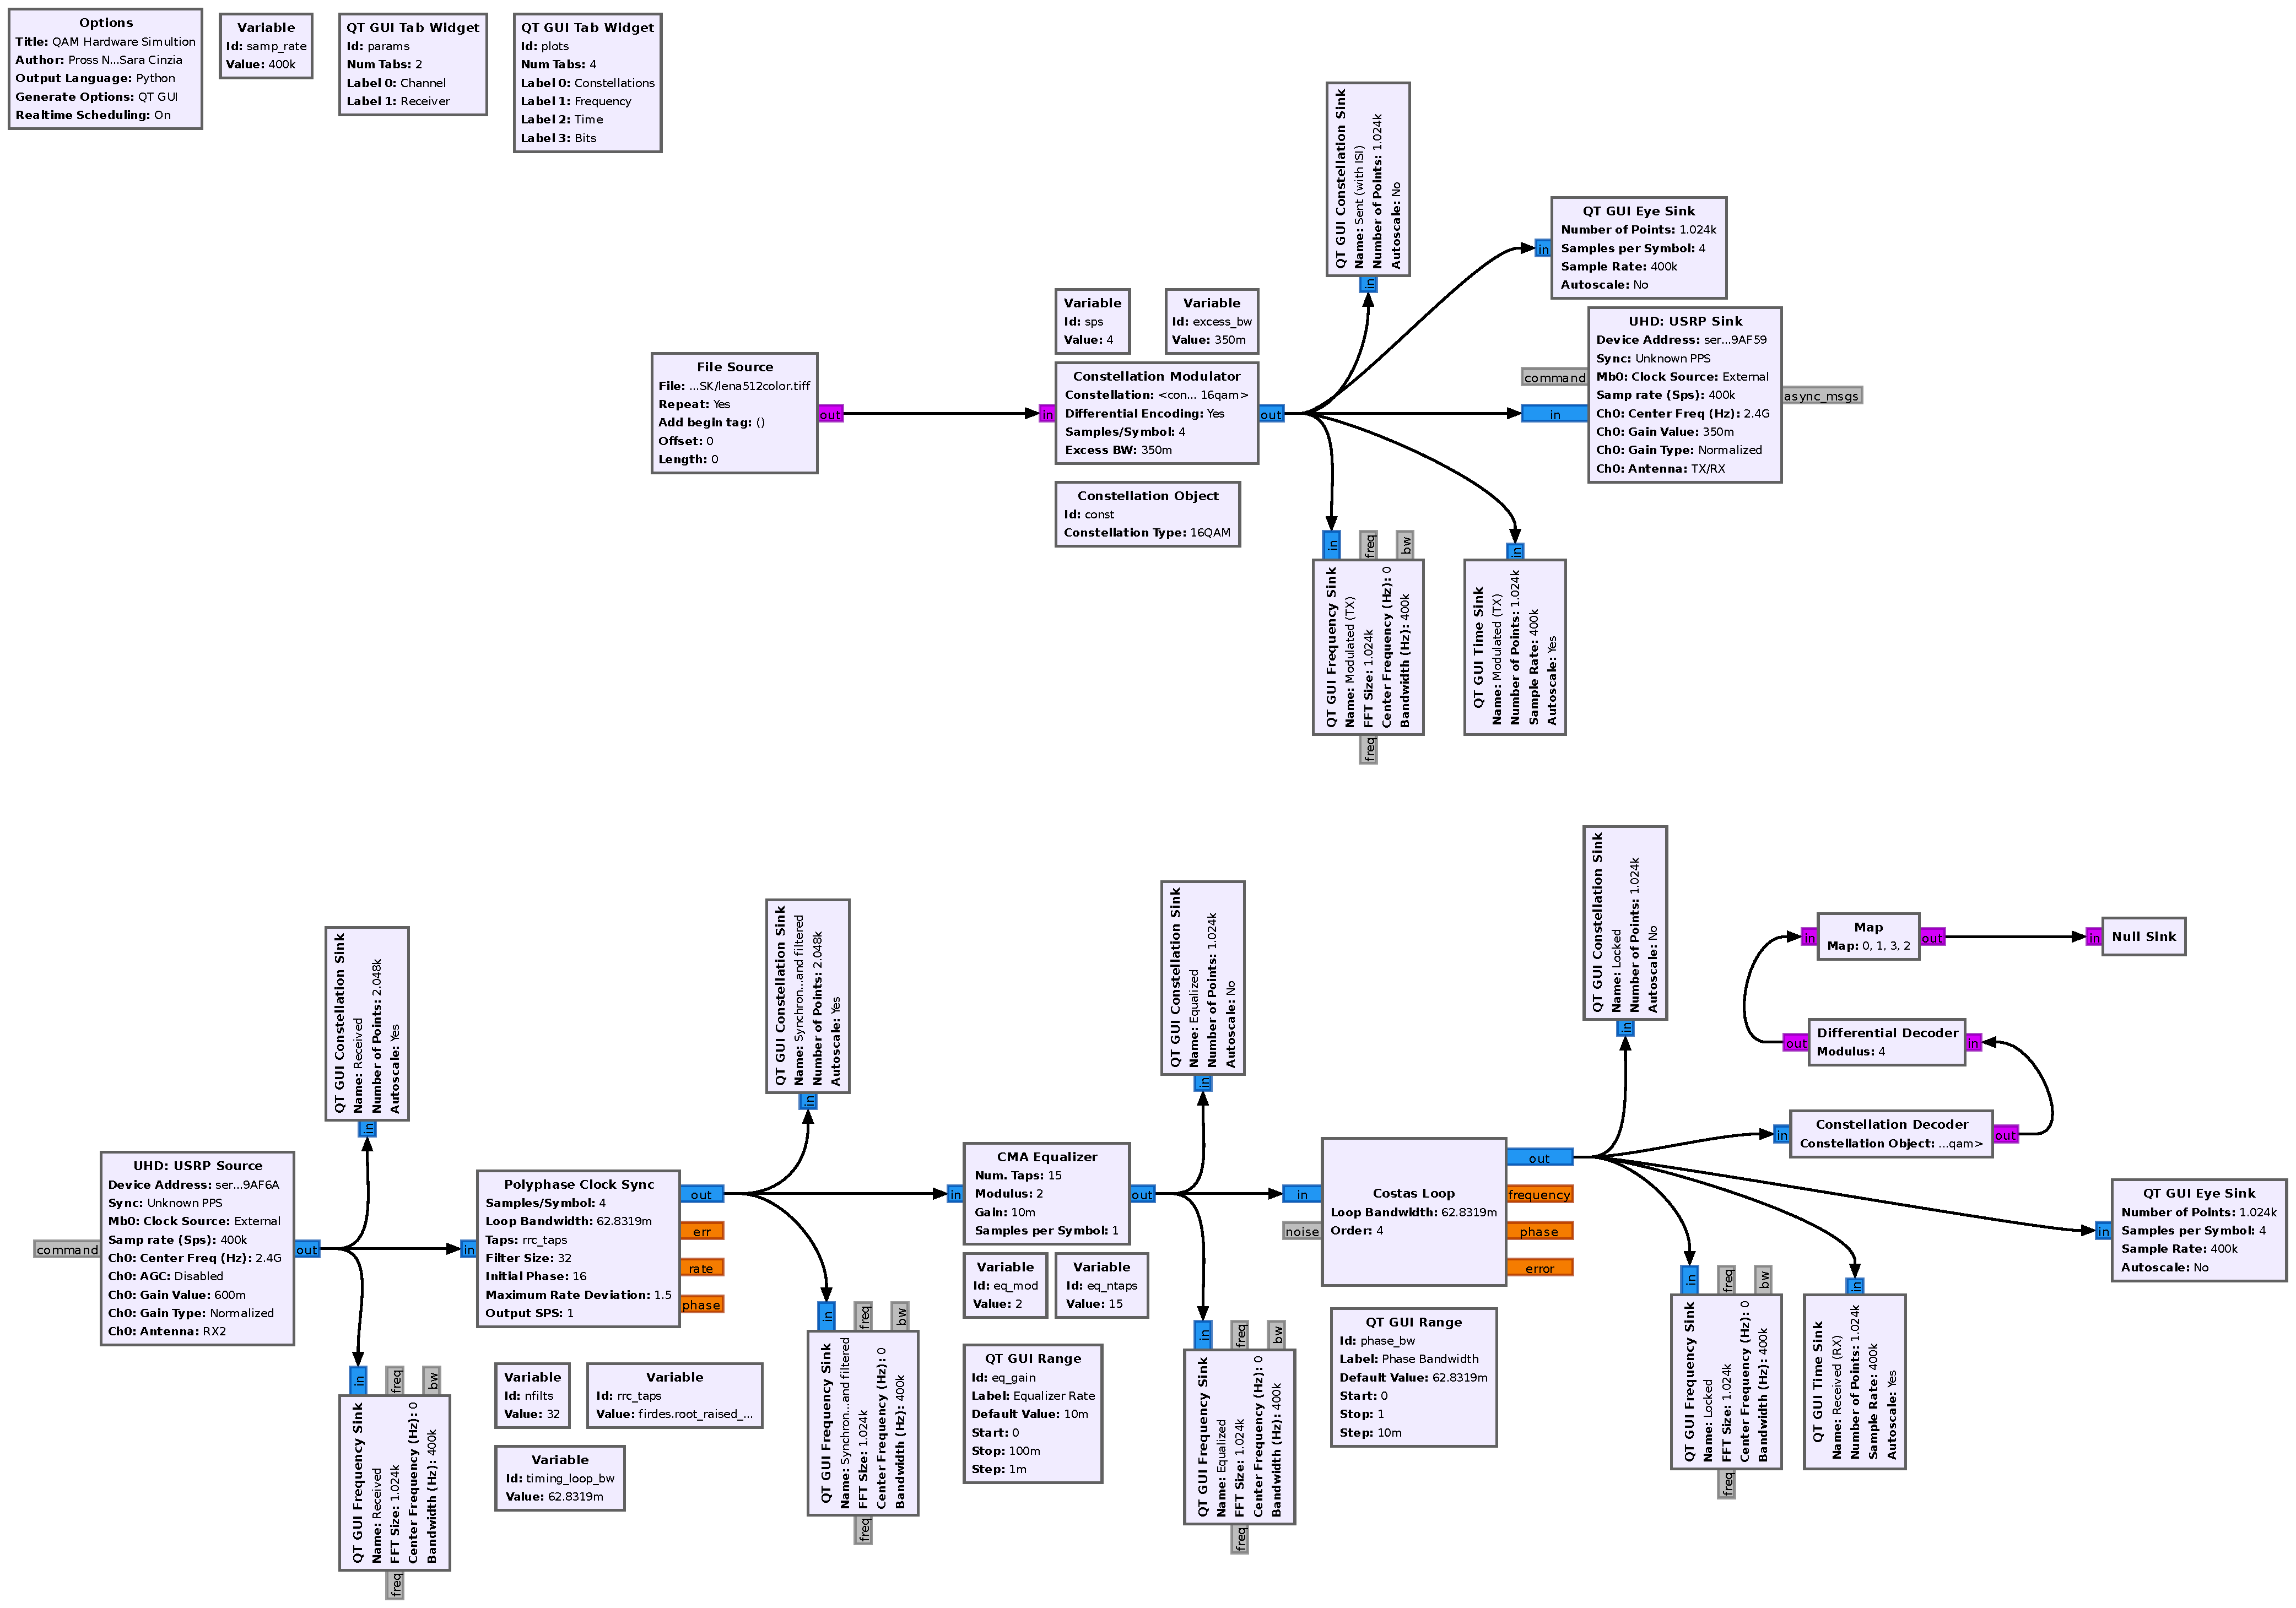
\includegraphics[width=\linewidth]{./figures/pdfs/qam_Hardware_1711.pdf}
	\caption{GNU Radio Blocks Hardware}
	\label{fig:simul16QAM_Hardware_Aufbau}	
\end{figure}

\begin{figure}
	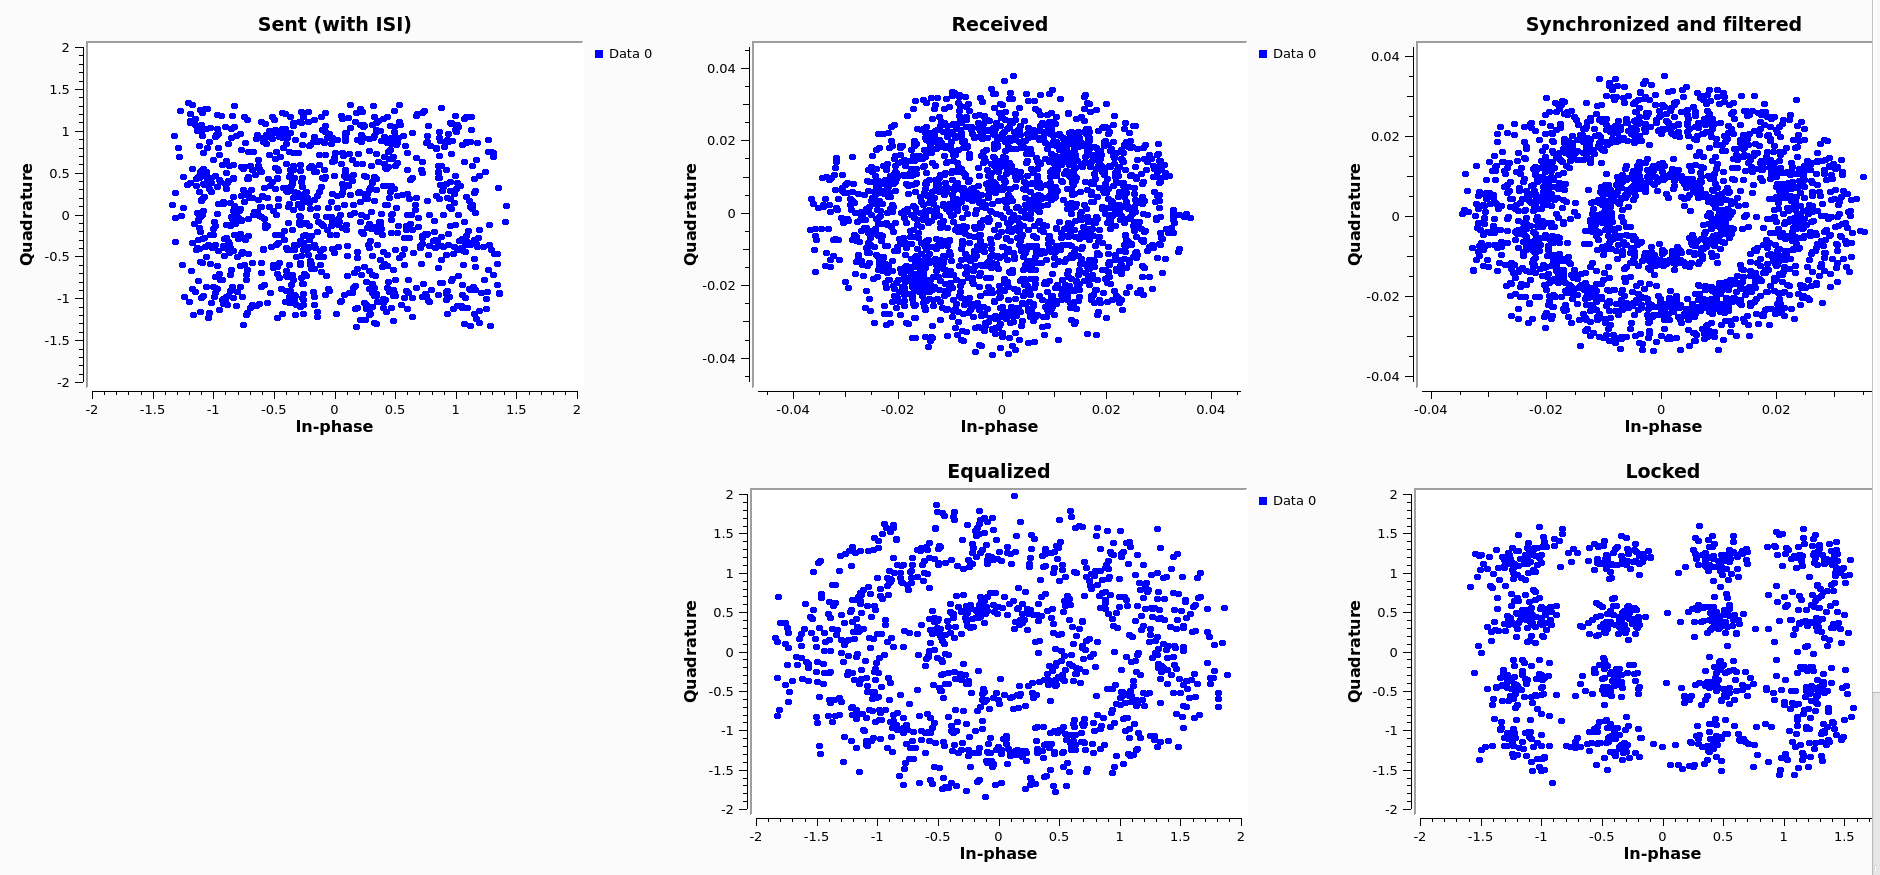
\includegraphics[width=\linewidth]{./figures/screenshots/QAM16_Hardware_1711.png}
	\caption{Hardware results}
	\label{fig:simul16QAM__Hardware}	
\end{figure}

% To Do: Picture of the setup

\begin{table}[]
	%To DO sepzifikationen ampssen / genauer? https://www.ettus.com/wp-content/uploads/2019/01/b200-b210_spec_sheet.pdf
	%https://kb.ettus.com/B200/B210/B200mini/B205mini#FAQ
	\centering
	\caption{USRP B210 specifications}
	\begin{tabular}{ll}
		\toprule
		Dimensions               & \(9.7 \times 15.5 \times 1.5\) cm \\
		Ports                    & 2 TX, 2 RX, Half or Full Duplex     \\
		RF frequencies           & from 70MHz to 6GHz                    \\
		Bandwidth                & 200kHz -- 56MHz                       \\
		External reference input & 10 MHz                                \\
		\bottomrule
	\end{tabular}
\label{tab:USRP B210 specifications}
\end{table}
